\subsection{Architektur}
\label{sec:Architektur}

Der Architekturentwurf des vorliegenden Projektes wurde bereits im \verweis{Architekturgrundlagen} als Ausgangsbasis zur Erläuterung der Grundlagen präsentiert. Aufbauend auf diesen Grundlagen wird der Architekturentwurf im Folgenden genauer betrachtet. Ausgangspunkt der folgende Darstellung ist die Architektur, die in \abbildung{Architektur} zu sehen ist.

\begin{figure}[htb]
\centering
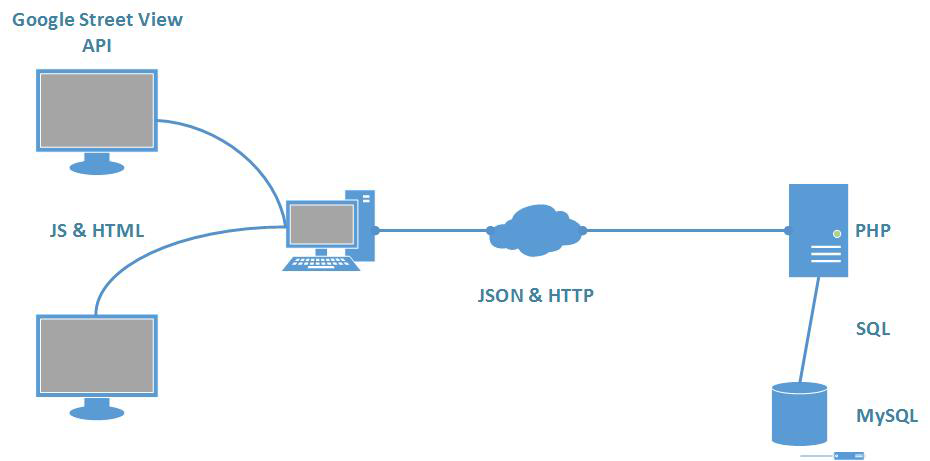
\includegraphics[width=1.0\textwidth]{Architektur.png}
\caption[Architektur der Anwendung]{Architektur der
Anwendung\protect\footnotemark}
\label{fig:Architektur}
\end{figure}
\footnotetext{Quelle: Eigene Darstellung}

Der dargestellte Architekturentwurf zeigt eine klassische Client-Server-Architektur. Das bedeutet die Architektur lässt sich in zwei Subsysteme aufteilen, die über definierte Schnittstellen kommunizieren können. Diese Kommunikation besteht immer in Form von Anfrage und Antwort. Ein Subsystem fragt dabei einen Dienst an, den das andere Subsystem anbietet. Das Clientsubsystem ist dabei definiert als das Subsystem, dass einen Dienst des Serversubsystems anfragt. Das Serversubsystem bietet damit einen Dienst an\footnote{\citet[S.~177]{rautenstrauch2002}}.

Im vorliegenden Projekt stellt das Serversystem vor allem Webdokumente und Schnittstellen (APIs) für das Clientsystem bereit. Zur Realisierung dieser Schnittstellen wird die Serverskriptsprache PHP und eine MySql-Datenbank eingesetzt. Bei der Anfrage eines Webdoukemnts wird auf dem Serversystem eine PHP-Routine durchgeführt und als Antwort ein HTML Dokument zurückgeliefert. Inhalt der PHP-Routine kann dabei eine Anfrage an die Datenbank sein, auf der aufbauend HTML dynamisch generiert wird.
Bei Anfragen an sogenannte Application Programming Interfaces (APIs) werden ebenfalls Informationen mit Hilfe von PHP aus der Datenbank gelesen und in einem definierten Format zurückgeliefert. Im Gegensatz zu Webdokumenten ist eine solche Schnittstelle (engl: interface) für den Informationsaustausch zwischen Programmen ausgelegt ist. Das Ausgabeformat der dargestellten Informationen ist aus diesem Grund nicht für menschliche Lesbarkeit optimiert.

Die Anfragen an den Server werden durch den Benutzer initiert und die zurückgelieferten Antworten werden interpretiert. Das Clientsystem ist dabei im vorliegenden Projekt der Internetbrowser eines Benutzers. Dieser löst durch das Aufrufen von Webseiten anfragen aus, der Server beantwortet diese und der Internetbrowser des Benutzers stellt das zurückgelieferte HTML dar. Eine solche Anfrage ist ein Anwendungsbeispiel für eine Anfrage nach einem Webdoukment. Darüber hinaus werden auf dem Client Routinen der Programmiersprache Javascript ausgeführt.
Durch Javascript können dabei Benutzerinteraktionen direkt auf dem Client verarbeiten werden. Das steigert die Performanz, da keine erneuten Anfragen an den Server geschickt werden müssen. Über diese Technologie ist auch die Google Street View API eingebunden. Diese erlaubt es 360-Grad-Fotos darzustellen und zu weiteren festgelegten Panoramas zu navigieren.